\chapter{Background}
\section{Projective Geometry}
\begin{figure}[h!]
   \centering
   \includegraphics[width=0.6\textwidth]{images/Projective.jpg}
   \caption{Visualization of projective geometry}
   \label{pics:proj}
\end{figure}

The projection of a world point $P_w \in \mathbb{R} ^ {3 \times 1}$ into the image frame requires the multiplication with the perspective projection matrix $M \in \mathbb{R} ^{3 \times 4}$ \citep{dawson1994simple}. $M$ is defined as the multiplication of the camera intrinsic matrix $K  \in \mathbb{R} ^{3\times3}$ with the rotation matrix $R \in \mathbb{R} ^{3 \times 3}$ and  horizontally concatenated translation vector $t \in \mathbb{R} ^{3 \times 1}$ of the camera in the world frame. To use these matrices, $P_w$ has to be converted into homogeneous coordinates by vertically appending a "$1$".
\begin{equation}
 \lambda \begin{pmatrix} u \\ v \\ 1 \end{pmatrix} = M \begin{pmatrix} X_w \\ Y_w\\ Z_w \\ 1 \end{pmatrix} = K \; [R \; | \; t] \begin{pmatrix} X_w \\ Y_w\\ Z_w \\ 1 \end{pmatrix} = K \begin{pmatrix} X_c \\ Y_c\\ Z_c \end{pmatrix}
  \label{eq:proj}
\end{equation}

The matrix $K$ containing the intrinsic parameters of the camera is shown in equation \ref{eq:instrinsics}, where $\alpha$ is the focal length in pixels and $(u_0, v_0)$ are the coordinates of the optical center, also known as the principal point, in pixels. If the pixels are not perfectly square, $\alpha_u$ and $\alpha_v$ will not have the same values. The focal length in pixels $\alpha_u$ or $\alpha_v$ can be converted into meters with the respective conversion factor $k_u$ or $k_v$. 

\begin{equation}
K = \begin{pmatrix} \alpha_u & 0 & u_0\\ 0 & \alpha_v & v_0 \\ 0 & 0 & 1 \end{pmatrix}
\; \; \; \; \;  \; \;  \; \; \alpha_i = k_i \cdot f,  \; \; \; i \in  \; \{u,v\}
  \label{eq:instrinsics}
\end{equation}
In the rest of the report, for clarity purposes, the focal length in pixels will be referred to as $f$ with the subscript of the according direction $\{u,v \}$.\\

If the camera's lens is distorted, this needs to be corrected, prior to the conversion of a world point to an image point, to be able to compute precise dimensional measurements. The two types of distortion are radial and tangential \citep{weng1992camera}. Different transformation equations must be applied to find the new coordinates of the undistorted image points for these two types of distortions.
\begin{figure}[h]
    \centering
    \subfigure[]{\includegraphics[width=0.36\textwidth]{images/rad_distortion.png}} 
    \subfigure[]{\includegraphics[width=0.48\textwidth]{images/tang_distortion.png}} 
    \caption{a) Solid lines: no distortion, dashed lines: radial distortion, where $a$: negative and $b$: positive, (b) Solid lines: no distortion, dashed lines: tangential distortion\citep{weng1992camera}}
    \label{pics:distort}
\end{figure}
\newpage







\section{Vanishing Points}
The world frame can be described by three mutually orthogonal axes. All lines running in the direction of one of these axes are parallel. When observing an image of the world, this property is no longer maintained. The lines are still perceived as straight but no longer parallel.

\begin{figure}[h!]
   \centering
   \includegraphics[width=0.5\textwidth]{images/vanishing.png}
   \caption{Vanishing points in a perspective image \citep{magee1984determining}}
   \label{pics:vanishing}
\end{figure}

 As can be seen in the perspective Figure \ref{pics:vanishing}, the lines parallel in a plane converge to one point, called vanishing point \citep{caprile1990using}. This property is reversible, meaning if two lines converge to a vanishing point, they are parallel in the world frame. 
When assuming perspective projection, every image contains three vanishing points $\{V_x, V_y, V_z \}$, which can lie outside of the image plane or even converge in infinity depending on the position of the camera with respect to the world frame. Any straight line that is parallel to the image plane has a vanishing point in infinity \citep{liu2010viewing}. The two vanishing points $\{V_x, V_y \}$ are referred to as horizontal vanishing points in Figure \ref{pics:vanishing}, and $V_z$ as the vertical vanishing point. A vanishing line is defined as a line that contains two vanishing points. Therefore in a perspective image, three vanishing lines exist. In a projective image, the horizon line is where all planes parallel to the ground plane meet. 







\chapter{General Approach } \label{sec:general_approach}
When a camera is randomly attached at the front of a track driving vehicle, its pose relative to the preinstalled GPS shown in blue in Figure \ref{pics:goal} is unknown. To determine these six degrees of freedom, three for the position and three for the orientation, a combination of visual-, map-, and GPS information is leveraged. With this knowledge, we close the circle, from the world frame to the camera frame, via the GPS and back.

\begin{figure}[h!]
   \centering
   \includegraphics[width=0.55\textwidth]{images/Goal.jpg}
   \caption{Relative poses between the world, GPS, and camera}
   \label{pics:goal}
\end{figure}

These six parameters are estimated in a multi-stage process, where they are computed over several frames and then averaged. The parameters are labeled as visualized in Figure \ref{pics:frame}. 

\begin{figure}[h!]
   \centering
   \includegraphics[width=0.85\textwidth]{images/frames.jpg}
   \caption{Labels of estimated parameters}
   \label{pics:frame}
\end{figure}

With prior knowledge, it is obvious that the monocular camera is attached at the front of the train and, therefore, must have a longitudinal offset to the GPS. As the GPS location is unknown, the magnitude of this parameter is obscure. This also holds for the other two translational camera offsets to the GPS. Therefore, the camera frame is initialized at the origin of the GPS frame. It is initialized with a rotation of $-90$° around the z-axis followed by a $-90$° intrinsic rotation around the x-axis. This way, the z-axis points forward, which is the standard way of defining a camera frame. Any estimate is made relative to the initial camera frame, where position estimates are added to the corresponding axis in the camera frame, and the rotations are extrinsically added to the camera frame. \\

The order in which the parameters are computed is of relevance, as some are dependent on others. This dependency is visualized in Figure \ref{pics:dep}. 

\begin{figure}[h!]
   \centering
   \includegraphics[width=0.7\textwidth]{images/depend.png}
   \caption{Visualization of parameter dependencies and their consequential order}
   \label{pics:dep}
\end{figure}
The process is subdivided into two steps; where first, the railway tracks are visually detected, and this information is then used to compute the parameters.







\newpage
\section{Rail Detection}
The basis of the pose estimation is a successful railway track detection. For our purposes, only a small part at the bottom of the image frame had to be detected. In this part of the image, the railway tracks can be approximated as straight lines \cite{nassu2011rail}, simplifying their detection.\\

Herefore, after having turned the current frame into a gray image, it was blurred with a $3 \times 3$ Gaussian kernel. For the determination of the most fitting edge detection algorithm, a comparison was done between the most commonly used algorithms, the Canny, LOG, Prewitt, Roberts, and Sobel edge detectors depicted in Figure \ref{pics:edge_detect}. We obtained the best results with the Canny edge detector, which has also been implemented by other authors \citep{namazi2019using}. 

\begin{figure}[h]
    \centering
    \subfigure[]{\includegraphics[width=0.49\textwidth]{images/Edge_Canny.jpg}} 
    \subfigure[]{\includegraphics[width=0.49\textwidth]{images/Edge_LOG.jpg}} 
    \subfigure[]{\includegraphics[width=0.49\textwidth]{images/Edge_Prewitt.jpg}}
    \subfigure[]{\includegraphics[width=0.49\textwidth]{images/Edge_Roberts.jpg}}
    \subfigure[]{\includegraphics[width=0.49\textwidth]{images/Edge_Sobel.jpg}}
    \caption{(a) Canny (b) LOG (c) Prewitt (d) Roberts (e) Sobel}
    \label{pics:edge_detect}
\end{figure}


After applying the Canny algorithm on the image, a probabilistic Hough Transform \citep{matas2000robust}, which allows searching for a predefined minimum length and maximal pixel gap, was performed. The resulting line candidates were further filtered with pre-knowledge of the train tracks geometry as proposed by Wang \citep{wang2015inverse}. This filter limited the admissible gradient for the detected rail and only allowed rails that crossed the bottom frame of the image. This last constraint had the benefit of filtering out railway tracks that ran parallel to the currently traveled-on tracks of the vehicle. As a final decision, when multiple line candidates for the rails were left, the candidates closest to the horizontal middle of the frame were chosen. This last decision was based on the fact that the standardized width of tracks is measured on the inside of the rails, which is leveraged later. If no appropriate candidates were determined the frame was skipped.
\newpage






\section{Parameters Estimation}
In the following section, the different approaches used to compute the individual parameters are described, where first, the translational ones are addressed, followed by the rotational ones.

\subsection{Height Offset Estimate}
The difference in height $h_{offset}$ between the GPS and camera was measured along the y-axis of the camera. Determining this height offset depended on having previously estimated $\varphi_{roll}$ of the camera. \\

With an approach inspired by Ross \citep{ross2010vision}, the radius $r$ was calculated in \text{Equation \ref{eq:r}} using the focal length in pixels $f_v$ along the vertical direction, the ratio $w_0$ between the perceived width of train tracks at the bottom of the image frame and the real-world standardized width of the train tracks $W$. This ratio was inserted into \text{Equation \ref{eq:h_c}} with the vertical field of view (FoV) of the camera, and the precomputed camera roll $\varphi_{roll}$ to obtain the height of the camera.

\begin{equation}
r = \frac{f_v\;  W}{w_0} 
\label{eq:r}
\end{equation}
\begin{equation}
 h_c = r  \; \; cos(\frac{\pi}{2}- \varphi_{roll} - FoV_v)
 \label{eq:h_c}
\end{equation}

\begin{figure}[h!]
   \centering
   \includegraphics[width=0.7\textwidth]{images/track_width.jpg}
   \caption{Geometry of perceived width of tracks and their real-world width}
   \label{pics:width_tracks}
\end{figure}

\begin{figure}[h!]
   \centering
   \includegraphics[width=0.6\textwidth]{images/height.jpg}
   \caption{Geometry used for the estimation of $h_{c}$ \citep{ross2010vision}}
   \label{pics:y_pos}
\end{figure}

Leveraging the elevation at the current train position \citep{digitales}, the $h_c$ was converted into the vertical height difference between the camera and GPS $h_{offset}$ in \text{Equation \ref{eq:y_pos}}.\\
\begin{equation}
h_{offset} = h_c + h_{elevation} - h_{GPS}
\label{eq:y_pos}
\end{equation}
\newpage


\subsection{Horizontal and Longitudinal Offset Estimate}
The estimation of the horizontal offset along the x-axis of the camera and the longitudinal offset along the z-axis of the camera was computed similarly. The difference in the visual perception to the known location of a distinctive landmark was leveraged. This process depends on all rotational estimates and the height offset of the camera.\\

As a distinctive object, many options existed, such as a turnout, curve, or pole, where the visual detection of a turnout has been researched \citep{qi2013efficient} \citep{ross2010vision} \citep{ross2012track} and the detection of curved tracks far ahead has also been done \citep{nassu2011rail}. The choice of the landmark was set on an electricity pole as it could be reduced to one fixed location at its contact point to the ground. Once the pole had been visually detected, the depth of its ground contact point in pixels had to be found, as it had to be converted into the GPS frame. Following this was a comparison between the visually detected pole in the GPS frame and its known location in the GPS frame.

\subsubsection{Visual Pole Detection}
To visually detect the electricity poles, HSV color ranges trimmed to the pole colors in different illumination cases were applied to the image. This was done, as a simple Hough Transform searching for vertical lines didn't suffice in finding lines that would run along the complete pole front. The top part of the poles was easily distinguished from the sky, but not so for the bottom part, depending on the pole's background. \\

The images were converted from an RGB color space into an HSV color space, separating the pixel color information into three layers: hue, saturation, and value. All pixels that fell within predefined HSV ranges were kept white, while all others were turned black. This process was followed by a component analysis that searched for groups of pixels with a certain area. This area was then compared to a predefined threshold to determine whether this group was desired. 

\begin{figure}[h]
   \centering
   \includegraphics[width=0.75\textwidth]{images/color_filtering.png}
   \caption{Image after application of HSV range filters and component analysis}
   \label{pics:component}
\end{figure}

The image with the remaining component had to be searched for the component representing the pole. This was done by searching the image for vertical lines with a Hough Transform that fulfilled constraints on its position. These constraints were set with the prior knowledge of the pole location next to the railway tracks. This filtered out any other objects that could have been detected, e.g., trees. 

This process only worked when the train was driving on a straight track, as only then were the poles observed as vertical and could be distinguished from the train tracks, which could have been included in the color-filtering process by chance. The component this vertical line belonged to was found by computing its distance to the centroid of the component and choosing the component with the smallest distance.

The ground contact point of the pole was then found by first finding the top pixel with a simple search through the component's pixels. The bottom pixel was chosen as the lowest one with the same $u$-coordinate as the top pixel. 

\subsubsection{Depth Computation}
In a setup with stereo cameras, performing the depth estimation is done by focusing on the same scene from different perspectives \citep{shan2011depth}. In others, with only a monocular camera, a laser could be used to compute the depth \citep{sun2010research}, \citep{yan2003mobile}. Some even apply a deep convolutional neural network in a monocular setup \citep{yin2017scale}. In our case, if the pole detection was successful, the lowest point should be on the ground, which can be leveraged to compute the depth $\lambda$ to convert the pixel to the camera frame \citep{namazi2022geolocation}.

\begin{equation}
 \lambda \begin{pmatrix} u \\ v \\ 1 \end{pmatrix} = K \begin{pmatrix} X_c \\ Y_c\\ Z_c \end{pmatrix} =  \begin{pmatrix} \alpha_u & 0 & u_0\\ 0 & \alpha_v & v_0 \\ 0 & 0 & 1 \end{pmatrix} \begin{pmatrix} X_c \\ Y_c\\ Z_c \end{pmatrix}
\label{eq:cam_coord}
\end{equation}
\\
\\
If the matrix notation of Equation \ref{eq:cam_coord} is written out in single equations and solved for the camera coordinates, we obtain the following three equations:

\begin{equation}
X_c = \frac{Z_c ( u - u_0)}{\alpha_u}  \; \; \; \; Y_c = \frac{Z_c ( v - v_0)}{\alpha_v} \; \; \; \; \lambda = Z_c 
\label{eq:inv_cam_coord}
\end{equation}
\\
\\
With the precomputed pose estimates of the camera, the homogeneous transformation matrix $H_{w/cam}$ from the camera to the world frame can be used to convert a point $P_c$ in homogeneous coordinates on the image frame to a point $P_w$ in homogeneous coordinates in the world frame:

\begin{equation}
 \begin{pmatrix} X_w \\ Y_w\\ Z_w \\ 1 \end{pmatrix}  = H_{w/cam}\begin{pmatrix}  X_c \\ Y_c\\ Z_c \\ 1\end{pmatrix} = \begin{pmatrix} h_1 & h_2 & h_3 & h_4\\ h_5 & h_6 & h_7 & h_8 \\ h_9 & h_{10} & h_{11} & h_{12} \\ 0 & 0 & 0 & 1 \end{pmatrix}  \begin{pmatrix} X_c \\ Y_c\\ Z_c \\ 1 \end{pmatrix}
\label{eq:world_coord}
\end{equation}
\\
\\
If Equation \ref{eq:inv_cam_coord} is plugged into Equation \ref{eq:world_coord}, the third row is taken, solved for $Z_c$ and our knowledge of $Z_w = h_{elevation}$ is used, we obtain Equation \ref{eq:depth}.

\begin{equation}
 Z_c = (h_{elevation} - h_{12})/( h_9  \frac{( u - u_0)}{\alpha_u} + h_{10}  \frac{(v - v_0)}{\alpha_v} + h_{11})
\label{eq:depth}
\end{equation}
\\
\\
As we know $\lambda = Z_c$, we can now use this depth to find the bottom point of the pole expressed in the GPS frame.


\subsubsection{Height Criterion}
As a condition of whether the pixels indicating the highest and lowest point of the pole are detected correctly and the frame can be used, the height of the pole in the world can be computed and compared to our prior knowledge of its height.

With our computed depth $\lambda$, we can find the distance of the pole from the base point of the camera $D'$ with our precomputed height estimate of the camera $h_c$ by simply applying Pythagoras theorem. When dividing this diagonal distance $D'$ by the cosine of $\alpha$, we obtain the horizontal distance $D$. 
\begin{equation}
D' = \sqrt{\lambda ^2 - h_c^2} \; \; \; \; \; D = \frac{D'}{cos(\alpha)}
\label{eq:horizontal_distance}
\end{equation}

\begin{figure}[h!]
   \centering
   \includegraphics[width=0.999\textwidth]{images/pole_views.jpg}
   \caption{a) Top view of the camera to pole geometry, (b) Side view of the camera to pole geometry}
   \label{pics:pole_depth}
\end{figure}

To determine the angle $\alpha$ visible in Figure \ref{pics:pole_depth} b), the distance $T$ seen in red in Figure \ref{pics:theta} can be determined and then converted to an angle by determining the percentage this distance takes up of the vertical $FoV_u$ \citep{namazi2022geolocation}.
\begin{equation}
T = u_0 - u_{pole}  \; \; \; \; \; \; \; \gamma = \frac{FoV_u}{2 \; u_0} \; \; \; \; \; \; \; \alpha = \gamma \cdot T
\label{eq:theta}
\end{equation}

\begin{figure}[h!]
   \centering
   \includegraphics[width=0.7\textwidth]{images/pole_theta.jpg}
   \caption{Exemplary image of parameters used to compute $\alpha$}
   \label{pics:theta}
\end{figure}

Using the horizontal distance $D$ and the height of the pole in pixels $h_{p}$, by subtracting the $u$-components of the highest from the lowest pixel of the pole, the height of the pole in the world frame $H$ can be computed. An aspect ratio can be set up, as the pole is an object that touches the ground \citep{euclid1943optics}. The approach used is the not-approximated approach proposed by Kar\citep{kar2015amodal}. The definition of the top pixel $P_{t}$ and bottom pixel $P_{b}$ given in Equation \ref{eq:pixel_coords} can be subtracted to get a definition for the height of the pole in pixels $h_{p}$ and solve it for the height of pole in meters $H$ in Equation \ref{eq:pixel_coords3}. 
\begin{equation}
P_{b} = f \frac{-h_c/D + tan(\varphi_{roll})}{1+(h_c/D) \; tan(\varphi_{roll})} \; \; \; \; \; \; \;
P_{t} = f \frac{-(h_c + H)/D + tan(\varphi_{roll})}{1+(h_c/D) \;tan(\varphi_{roll})}
\label{eq:pixel_coords}
\end{equation}

\begin{equation}
h_{p} = P_{t} - P_{b} 
\label{eq:pixel_coords2}
\end{equation}

\begin{equation}
H = \frac{h_{p} ( D + h_c \; tan(\varphi_{roll})) }{f_v}
\label{eq:pixel_coords3}
\end{equation}
\\


This height $H$ can be compared to the prior knowledge of the pole's height. If their difference is over a predefined threshold, this estimate can be discarded. The threshold can be set depending on how precise the previous estimates of the relative camera pose are.



\subsubsection{Horizontal Offset Estimate}
After a successful pole detection and depth computation, the horizontal offset $hl_{offset}$ can be computed. For this, after the visually detected ground contact point of the pole is expressed in the GPS frame and the same for the known location of the pole, their y-coordinates can be subtracted from each other:

\begin{equation}
hl_{offset} = _{GPS} y_{cam} - _{GPS} y_{world}
\label{eq:x_pos}
\end{equation}

\begin{figure}[h]
   \centering
   \includegraphics[width=0.45\textwidth]{images/horizontal.jpg}
   \caption{Geometry used to detect $hl_{offset}$ between camera and GPS}
   \label{pics:x_pos}
\end{figure}



\subsubsection{Longitudinal Offset Estimate}
The same holds for the longitudinal offset $l_{offset}$. As the camera is located at the front of the vehicle, meaning in front of the GPS, the x-coordinate of the object seen from the camera would be smaller than its actual x-coordinate in the GPS frame. This difference is used to compute the longitudinal offset between the camera and GPS.

\begin{equation}
l_{offset} = _{GPS} x_{world} - _{GPS} x_{cam}
\label{eq:z_pos}
\end{equation}

\begin{figure}[h!]
   \centering
   \includegraphics[width=0.5\textwidth]{images/longitud.jpg}
   \caption{Geometry used to detect $l_{offset}$ between camera and GPS}
   \label{pics:z_pos}
\end{figure}
\newpage





\subsection{Roll and Pitch Offset Estimate}
These two estimates are computed by leveraging the properties of the vanishing point in the image. As a rail has a width and the railway detection can have some slight variations, to make the location of the vanishing point more robust than simply taking the point where the two detected railway tracks intersect, the following process is proposed.

\subsubsection{Vanishing Point Detection}
\begin{figure}[h]
   \centering
   \includegraphics[width=1\textwidth]{images/vanish.jpg}
   \caption{a) $P_{v_0}$ at linearly extended railway tracks, (b) additional lines converging to the horizontal vanishing point}
   \label{pics:x_angle}
\end{figure}


The intersection of the detected railways, denoted as $P_{v_0}$, is utilized as prior for the vanishing point, as depicted in Figure \ref{pics:x_angle} a). However, to improve robustness, additional straight lines, represented by the orange lines in Figure \ref{pics:x_angle} b) that should converge to the same vanishing point, are incorporated into its calculation. The enlarged portion of Figure \ref{pics:x_angle} b) illustrates how the new vanishing point, denoted as $P_{v}$, is determined by taking the midpoint of the prior vanishing point $P_{v_0}$ and the intersection point $P_{int}$ of the newly added orange lines, both represented in blue and green respectively. To differentiate between lines converging to the various vanishing points present in an image, only those lines that intersect in close proximity to $P_{v_0}$ are used. This method also has the added benefit of excluding lines from, for example, junction tracks that could potentially interfere with accurate vanishing point detection.
\newpage

\subsubsection{Roll Offset Estimate}
In Equation \ref{eq:x_angle}, the height of the vanishing point $v_p$ is taken to compute the roll together with the middle of the vertical height of the image $v_0$ and the focal length $f_v$ in pixels in the vertical direction as proposed by Ross \citep{ross2010vision}.
\begin{equation}
\varphi_{roll} = arctan(\frac{v_0 - v_p}{f_v}) 
\label{eq:x_angle}
\end{equation}

\begin{figure}[h]
    \centering
    \subfigure[]{\includegraphics[width=0.55\textwidth]{images/X_angle1.jpg}} 
    \subfigure[]{\includegraphics[width=0.3\textwidth]{images/roll.jpg}} 
    \caption{a) Visualization of offset $h$ and vanishing point, (b) visualization of focal length $f$ and $\varphi_{roll}$}
    \label{pics:x_angle2}
\end{figure}







\subsubsection{Pitch Offset Estimate}
For the pitch offset, the difference $w$ between the $u_p$-coordinate of the vanishing point and the horizontal middle line of the image $u_0$ is detected. This is then converted into an angle with the focal length $f$. 
\begin{equation}
\theta_{pitch} = arctan(\frac{u_p - u_0)}{f_u}) 
\label{eq:y_angle}
\end{equation}

\begin{figure}[h]
    \centering
    \subfigure[]{\includegraphics[width=0.6\textwidth]{images/Y_angle.jpg}} 
    \subfigure[]{\includegraphics[width=0.3\textwidth]{images/pitch.jpg}} 
    \caption{a) Visualization of offset $w$ and vanishing point, (b) visualization of focal length $f$ and $\theta_{pitch}$}
    \label{pics:y_angle2}
\end{figure}


\newpage
\subsection{Yaw Offset Estimate}
For this estimation, a new Hough Transform of the image was computed with a smaller minimum line length. The idea was to detect the top and bottom contouring lines of the wooden sleepers between the railway tracks seen in Figure \ref{pics:z_angle} in red. The candidate lines obtained were further filtered to be valid if their gradient was in a limited range, based on the assumption that the camera was reasonably positioned to have a low rotational angle around this axis. Additionally, only lines were accepted that were found within a predefined range of the horizontal middle of the detected railway tracks. The gradient of all valid candidate lines was computed and averaged to obtain $\psi_{yaw}$.

\begin{figure}[h!]
   \centering
   \includegraphics[width=0.8\textwidth]{images/yaw.jpg}
   \caption{Geometry used for the estimation of $\psi_{yaw}$}
   \label{pics:z_angle}
\end{figure}






\chapter{Results}

The approach proposed above was applied to two pre-existing data sets of a Tatra-tram driving in Potsdam, Germany. This information led to the knowledge of the standardized railway track width of 1.435m, the height of the tram of 3.1m, and its width of 2.2m \citep{strassmichael},\citep{tram2000}. These two data sets were from two cameras attached at the front of the tram, which gave us some prior knowledge of the accuracy of the obtained estimates. For other pre-existing data sets, there is a complete lack of ground truth.

\begin{figure}[h!]
   \centering
   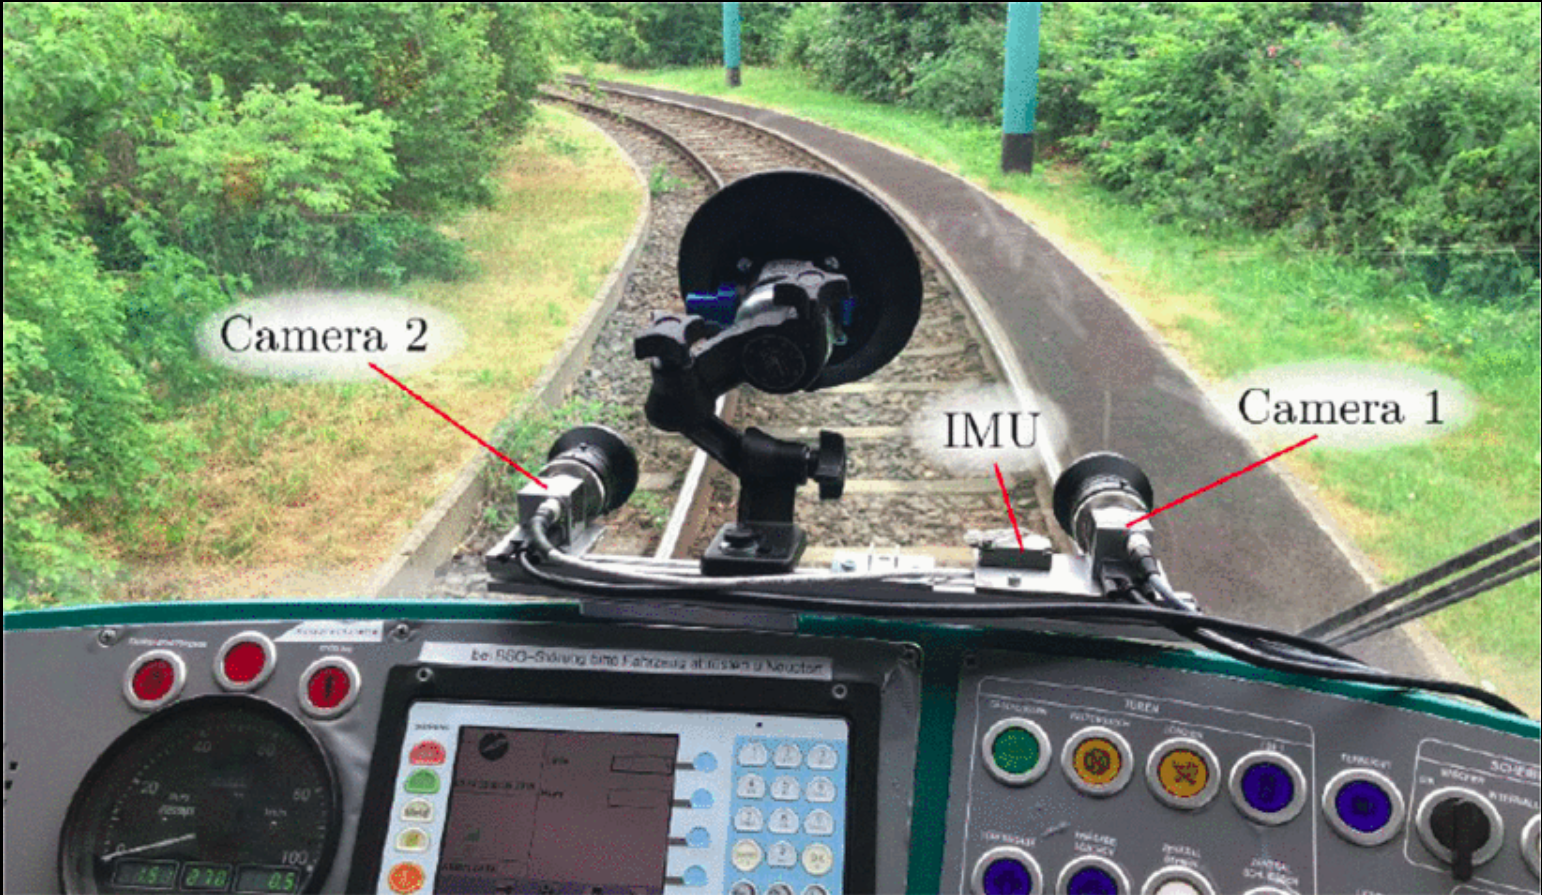
\includegraphics[width=0.99\textwidth]{images/camera_setup.png}
   \caption{Setup of the two cameras used for methodology validation}
   \label{pics:setup}
\end{figure}
\newpage




\section{Height Offset Estimate}
Table \ref{tab:stats_h_offset} shows the statistical summary, meaning the median and variance of the $h_{offset}$ across 70 frames of each camera. \\
\begin{table}[h!]
\centering
\begin{tabular}{c c c}
% \toprule
\textbf{h$_{offset}$}  & \textbf{Camera 1} & \textbf{Camera 2} \\
\midrule
% \textbf{Mean} & -1.05 m & -0.99 m \\
% \midrule
\textbf{Median [m]} & $-1.05$ & $-0.99 $ \\
% \midrule
\textbf{Variance [m$^2$]} & $5.1 * 10^{-4}$ & $2.99 * 10^{-4} $ \\
% \midrule
\textbf{Sample Number} & $70$ & $70$ \\
\bottomrule
\end{tabular}
\caption{Statistical summary of $h_{offset}$ of Camera 1 and Camera 2}
\label{tab:stats_h_offset}
\end{table}

Due to the lack of ground truth, the only manner of validating the height offset estimates of the individual cameras was by comparing the computed height of the camera with the ground truth camera setup height of 1.55m. The error was computed with Equation \ref{eq:error_height}, where the absolute difference to the ground truth was calculated.

 \begin{equation}
Error = |1.55 - h_c|
\label{eq:error_height}
\end{equation}

\begin{figure}[h!]
   \centering
   \includegraphics[width=0.5\textwidth]{images/setup1.jpg}
   \caption{Visualization of camera height for setup}
   \label{pics:setup3}
\end{figure}

In Table \ref{tab:y}, the individually computed values of the camera's height are presented. Compared to each other, they differ by 0.03m, where Camera 1 is 0.05m off of the ground truth value, and the error of Camera 2 is 0.13m.\\

\begin{table}[h!]
\centering
\begin{tabular}{c c c}
% \toprule
\textbf{Camera height}  & \textbf{Camera 1} & \textbf{Camera 2} \\
\midrule
\textbf{Median [m]} & $1.48$ & $1.42$ \\
\textbf{Error [m]} & $0.07$ & $0.13$ \\
\bottomrule
\end{tabular}
\caption{Median of camera heights and corresponding error}
\label{tab:y}
\end{table}

 \newpage
To get the required height offset estimate, the height of the GPS off the floor was subtracted from the camera height. To determine this height, the floor elevation at the current position was leveraged. As the GPS is rigidly mounted on the tram, this value should be stable and would only vary depending on the preciseness of the floor elevation data. In Table \ref{tab:gpsheight}, the statistics on the GPS height computed over 700 frames are visualized.

\begin{table}[h]
\centering
\begin{tabular}{cc}
\textbf{} & \textbf{GPS height from floor} \\
\midrule
\textbf{Median [m]} & $0.43 $ \\
\textbf{Variance [m$^2$]} & $9 * 10^{-4} $\\
\textbf{Sample Number} & $700$\\
\bottomrule
\end{tabular}
\caption{Statistical summary of GPS height from floor}
\label{tab:gpsheight}
\end{table}
\newpage






\section{Horizontal Offset Estimate}
Likewise, without the ground truth values, the manner of validating the horizontal offset estimates $hl_{offset}$  of the two cameras was by leveraging the known distance of 0.3m between them. By subtracting the horizontal offset values of the two cameras, this difference was compared to the known gap. Additionally, with the known width of the tram of 2.2m, a permissible upper bound on the estimates could be placed.
\begin{figure}[h!]
   \centering
   \includegraphics[width=0.35\textwidth]{images/setup2.jpg}
   \caption{Visualization of the distance between the two cameras in setup}
   \label{pics:setup2}
\end{figure}

Table \ref{tab:stats_hl_offset} shows the statistical summary of the horizontal offset estimate of both cameras. With these values, the cameras were separated by a distance of 0.31m. 

\begin{table}[h!]
\centering
\begin{tabular}{ccc}
\textbf{hl$_{offset}$}  & \textbf{Camera 1} & \textbf{Camera 2} \\
\midrule
\textbf{Median [m]} & $1.28$ & $0.97$ \\
\textbf{Variance [m$^2$]} &  $ 3 * 10^{-3}$ & $0.05$ \\
\textbf{Sample Number} & 3 & 5 \\
\bottomrule
\end{tabular}
\caption{Statistical summary of $hl_{offset}$ of Camera 1 and Camera 2}
\label{tab:stats_hl_offset}
\end{table}
\newpage







\section{Longitudinal Offset Estimate}

\begin{figure}[h!]
   \centering
   \includegraphics[width=0.4\textwidth]{images/long_results.jpg}
   \caption{Visualization of distance between camera and GPS for setup}
   \label{pics:long_truth}
\end{figure}

The longitudinal offset estimate was difficult to validate as no range on its value was known. The only prior knowledge given by the camera setup was, that these values should be of the same magnitude, as the two cameras were installed next to each other.\\

The following Table \ref{tab:stats_long} represents the statistical data of the estimates made. By comparing the median of the $l_{offset}$ estimates, the cameras had a difference of $0.44m$.

\begin{table}[h!]
\centering
\begin{tabular}{c c c}
  & \textbf{Camera 1} & \textbf{Camera 2} \\
\midrule
\textbf{Median [m] } & $0.04$ & $0.48$ \\
\textbf{Variance [m$^2$]} &  $3.2 * 10^{-2}$ & $2.5 * 10^{-2}$ \\
\textbf{Sample Number} & 3 & 4 \\
\bottomrule
\end{tabular}
\caption{Statistical summary of $l_{offset}$ of Camera 1 and Camera 2}
\label{tab:stats_long}
\end{table}






\newpage
\section{Rotational Estimates}
The computed rotational estimates were compared to the ground truth in two different manners, which will be explained in the following two sections.\\

In both cases, the rotational estimates were converted into one rotation matrix, which was then transformed into three Euler angles using a predefined order. The same was done for the ground truth rotation matrix. The obtained three Euler angles per rotation matrix were compared to each other by taking their respective squared difference. This calculation is visualized in Equation \ref{eq:rot_euler}, where the values from the ground truth have a subscript $t$, and the computed estimates a \text{subscript $e$}. 
 \begin{equation}
Error = \sqrt{(x_t - x_e)^2 + (y_t - y_e)^2 +(z_t-z_e) ^2}
\label{eq:rot_euler}
\end{equation}


\subsection{Rotation leveraging IMUs}
\begin{figure}[h!]
   \centering
   \includegraphics[width=0.6\textwidth]{images/rot_setup.jpg}
   \caption{Visualization of rotations $R_0$, $R_L$ and $R_R$}
   \label{pics:rotsetup}
\end{figure}
This first validation method compared the ground truth rotation matrix from the GPS to the respective camera. In detail, this entails the single steps from the GPS to the GPS-IMU, to the camera-IMU, and then to the corresponding camera. The rotation angle from the GPS to the GPS-IMU is zero, which is expressed as an identity matrix. The rotation from the GPS-IMU to the camera-IMU is defined as $R_0$, and the rotation from the camera-IMU to the left camera as $R_L$ and $R_R$ for the right camera.

\begin{equation}
R_{TOT} = R_{GPS/ GPS \;IMU} \; R_0  \; R_i \; \; \; \; \; \; \; \; i \in \{ L, R\}
\label{eq:rot}
\end{equation}

With this approach of comparing the estimated rotation per camera to the ground truth, the error in Table \ref{tab:rot1} was obtained and calculated with Equation \ref{eq:rot_euler}.

\begin{table}[h!]
\centering
\begin{tabular}{ccc}
% \toprule
  & \textbf{Camera 1} & \textbf{Camera 2} \\
\midrule
\textbf{Error [°]} & $1.1$ & $2.44$ \\
\bottomrule
\end{tabular}
\caption{Rotation errors of Camera 1 and Camera 2}
\label{tab:rot1}
\end{table}







\newpage
\subsection{Relative Rotation between Cameras}
\begin{figure}[h!]
   \centering
   \includegraphics[width=0.4\textwidth]{images/rot_setup2.jpg}
   \caption{Visualization of relative rotation from Camera 2 to Camera 1}
   \label{pics:rotsetup2}
\end{figure}
The second manner of validating the rotational values was by computing the relative rotation from the left camera to the right camera and comparing it to the ground truth attained from the calibration report of the camera setup. Table \ref{tab:rot2} presents the computed error by using the same error metric as applied to the first validation manner.

\begin{table}[h!]
\centering
\begin{tabular}{cc}
% \toprule
  & \textbf{Camera 1 to Camera 2} \\
\midrule
\textbf{Error [°]} & $0.49$ \\
\bottomrule
\end{tabular}
\caption{Rotation error of Camera 1 and Camera 2}
\label{tab:rot2}
\end{table}


\subsection{Statistics on Roll, Pitch, and Yaw}
As in the previous validation manners, the individually computed rotational values roll, pitch, and yaw were inspected as a whole in a rotation matrix. Table \ref{tab:indiv_rot} gives an overview of the statistics of the single values. Presented are the median and the variance over a certain sample number. The wooden sleepers needed for the yaw weren't found as often as the vanishing point needed for the roll and pitch, leading to a lower sample number.


\begin{table}[h!]
\centering
\begin{tabular}{c c c c}
% \toprule
& & \textbf{Camera 1} & \textbf{Camera 2} \\
\midrule
\textbf{Roll} &  & & \\
% \textbf{Roll} & Mean & $-0.33$°& $0.77$°\\
% \midrule
& Median [°] & $-0.31$&$ 0.73$\\
% \midrule
&Variance & $4.46 *10^{-4}$ & $4.59*10^{-4} $\\
&Sample Number & $70$ & $70 $\\
\midrule
% \textbf{Pitch} & Mean & $-0.49$° & $1.57$°\\
\textbf{Pitch} & &  & \\
% \midrule
&Median [°]& $-0.48$ & $1.57$\\
% \midrule
&Variance & $9.92 * 10 ^{-5}$ & $7.89 * 10 ^{-5}$\\
&Sample Number & $70$ & $70 $\\
\midrule
\textbf{Yaw} &  & & \\
% \textbf{Yaw} & Mean & $0.0$°& $0.0$°\\
% \midrule
&Median [°] & $0.0$& $0.0$\\
% \midrule
&Variance &$ 0$ & $0$\\
&Sample Number & $30$ & $30$ \\
\bottomrule
\end{tabular}
\caption{Statistical summary of roll, pitch, and yaw of Camera 1 and Camera 2}
\label{tab:indiv_rot}
\end{table}










\newpage
\section{Railway Map Projection}
A method to ascertain all estimated parameters at once was to project the known coordinates of the railway tracks into the image with the computed pose. The accuracy of the estimated pose could be determined by the degree of alignment between the projected railway tracks and those present in the image.\\

The left side of Figures \ref{pics:proj_cam0} and \ref{pics:proj_cam1} feature the projected railway tracks from the map without any pose estimates, whereas on the right-hand side, the figures depict the projected railway tracks using the respective pose. \\

\begin{figure}[h]
    \centering
    \subfigure[]{\includegraphics[width=0.49\textwidth]{images/cam0_no_pose.png}} 
    \subfigure[]{\includegraphics[width=0.47\textwidth]{images/cam0_projection.png}} 
    \caption{Projection of railway track into the frame of Camera 1 (a) with no estimated pose, (b) with estimated pose}
    \label{pics:proj_cam0}
\end{figure}

\begin{figure}[h]
    \centering
    \subfigure[]{\includegraphics[width=0.47\textwidth]{images/cam1_no_pose.png}} 
    \subfigure[]{\includegraphics[width=0.49\textwidth]{images/cam1_projection.png}} 
    \caption{Projection of railway track into the frame of Camera 2 (a) with no estimated pose, (b) with estimated pose}
    \label{pics:proj_cam1}
\end{figure}




\newpage
In order to determine which parameters were most in need of adjustment, they were altered manually and used to project the railway tracks into the image. Analysis of both camera views revealed that possibly only two parameters required larger modifications. In both cases, this specifically meant a reduction in horizontal offset by approximately $0.3$m and an increase in camera pitch rotation angle by approximately $2$° for Camera 1 and approximately $4$° for Camera 2, to achieve the projection seen in Figure \ref{pics:correct_proj}.

\begin{figure}[h]
    \centering
    \subfigure[]{\includegraphics[width=0.49\textwidth]{images/cam1_correct_projection.png}} 
    \subfigure[]{\includegraphics[width=0.48\textwidth]{images/camera0_corrected_projection.png}} 
    \caption{Railway projection with corrected parameters (a) for Camera 2, (b) for Camera 1}
    \label{pics:correct_proj}
\end{figure}





\newpage
\chapter{Conclusion}

This thesis presents a comprehensive method for determining the relative pose between a monocular camera mounted at the front of a track vehicle to a preinstalled GPS. This method can be applied online and also to pre-existing data sets. The process of parameter determination was performed in a multi-staged fashion. The horizontal vanishing point found at the intersection of the railway tracks was utilized for the roll, pitch, and height estimates. For the other parameters, distinctive landmarks were leveraged, wooden sleepers for the yaw, and electricity poles for the horizontal and longitudinal estimates. As there is a complete lack of ground truth, the proposed approach was applied to two data sets for which some prior knowledge of their parameters existed. \\

The results were, on the one hand, validated with prior knowledge of the translational estimates and by leveraging the IMUs for the rotational estimates. On the other hand, they were validated as a whole in the degree of alignment of the railway track projections with the estimated pose to the railway tracks seen in the image. \\

When analyzing the results of the rotational estimates with the IMUs, distinguishing the source of error between the three angles was rather difficult as these three values were transformed into one matrix. The rotation error was found to be smaller for Camera 1 than for Camera 2. This is thought to partially originate in a less precise roll estimate for Camera 2, as the thereon-depending height estimate was also less accurate. When validating the rotation results with the railway projection, both cameras seemed to also have an error in their pitch. The reason for the incorrect roll and pitch estimates lies in the inaccurate vanishing point detection, which would originate in a faulty railway track detection. The railway tracks have a width, and depending on their detection, we have slight variations.\\


When examining the translational estimates, the height offset error for Camera 1 was $0.07$m and $0.13$m for Camera 2. A source of error could be the dependency on elevation data, which had a precision of 1m. The impact of this error was analyzed by observing the variance of the GPS height, which should be zero but had a value of $9*10^{-4}$ m$^2$. Additionally, the error of the camera roll propagated to this estimate.\\

Even though the difference between the horizontal offset estimates nearly corresponded to the known gap, this didn't help decipher whether these two values should be shifted more to the left or right. What became evident with the manually corrected railway projection was that, indeed, they needed to be moved by approximately $0.3$m. This error is suspected to originate in their dependency on the roll, pitch, yaw, and height offset estimates.\\

The longitudinal offset estimates were found to be less precise, as they were dissimilar by a value of $0.4$m. This can also be explained by their dependency on all five prior pose estimates. Even a slight change in roll and pitch had a large impact on the depth computation needed for this parameter. As we observed in the manually corrected projection, the pitch for both cameras was off, and additionally, the roll was slightly off as the thereof resulting height estimates were also slightly amiss.\\

Generally, it can be concluded that with precise vanishing point detection, the error in roll and pitch can be decreased. This would lead to smaller propagated errors, impacting the height-, horizontal- and longitudinal offsets. Nevertheless, when comparing the degree of alignment of the tracks a large improvement was seen. Adding a safety margin to the projected railways, the possibility of the methods application in the real world exists.\\

In future work, an option to improve the visual electricity pole detection could be to train a convolutional neural network to obtain the optimal set of hue, saturation, and value ranges. If this were to be precise, then the detection of the longitudinal offset wouldn't have to be restricted to situations where the track vehicle drives on straight tracks, and the estimate could be computed more often. Additionally, a prior frame evaluation could be done to select keyframes automatically. This could be implemented in the manner proposed by Schneider \citep{schneider2017visual}, where a score is computed depending on the amount of information visible in a frame. When the score passes a predefined threshold, the frame is marked as a keyframe. 
